\section{SeismicDarts}\label{sec:SeismicDarts}

The SeismicDart combines a geophone (GS-100) with the fins and body of a lawn Jart\textsuperscript{TM}, using a 3D-printed chamber that encloses a WiFi-enabled microcontroller (particle.io Photon\textsuperscript{TM}) as shown in Fig.~\ref{fig:Smart_Dart_overview}. 
The center of the chamber is slotted to fit a wooden plate holding an accelerometer that transmits data wirelessly through the microcontroller. 
The centered accelerometer card allows placing the microcontroller and battery on opposite sides, balancing the dart.
Designs and instructions to build a SeismicDart are available at \cite{Victor2016Thingiverse}.



\begin{figure} \centering
{\includegraphics[width=\columnwidth]{Smart_Dart_overview.pdf}}
\caption{Components of the SeismicDart sensor: a lawn  Jart\textsuperscript{TM} fin, particle.io Photon\textsuperscript{TM}  micro-controller, 3D printed protective casing, and a geophone} 
\label{fig:Smart_Dart_overview}
\end{figure}

%%%%%%%%%%%%%%%%%%%%%%%%%%%%%%%%%%%%%%% 
\subsection{Experiments} 
The following sections compare SeismicDart performance.
\subsubsection{ Drop tests in different soils}  
This experiment varied the drop height and measured the penetration depth in four types of soil. 
Proper planting of a geophone requires good contact with the soil, in a vertical position. 
To determine the minimum deployment height for good planting, each trial measured the penetration depth and angular deviation from vertical. 
This experiment compared drop tests as a function of soil type. 

To determine how SeismicDarts perform in different soils, this experiment measured penetration into four soil types. Each trial was performed by holding the darts at the tip opposite to the spike in a vertical position and releasing them at varying heights into 19 liter (5 gal.) buckets of soil.
 Penetration depth and angular deviation were measured. To measure penetration depth, the buried darts were marked where the spike met the soil, the dart was then pulled from the soil, and the distance from the spike tip to the marking was measured with calipers. The angular deviation was recorded using the accelerometer inside the dart. The soil types were categorized by their compression strength, in kg/cm$^3$, measured using a soil pocket penetrometer (CertifiedMTP). Measurements for compression strength vary with small deviation in measurement location, so we repeated this measurement 10 times at 10 different locations in each soil type and took the average. These values for soil compression strength and a graph displaying heights vs. penetration depth are displayed in Fig.~\ref{fig:DepthPlotIndoors}, and a graph of angular deviation is in Fig.~\ref{fig:AnglePlotIndoors}. 
  The experiment shows that increasing drop height increases penetration on all soils tested.
  Also, darts dropped in quiescent air remain vertical if they penetrate the soil.


\begin{figure} \centering
{\includegraphics[width=\columnwidth]{indoor_depth_plot.pdf}}
\caption{Drop height vs. penetration depth in four soil types.} 
\label{fig:DepthPlotIndoors}
\end{figure}

\begin{figure} \centering
{\includegraphics[width=\columnwidth]{indoor_angle_plot.pdf}}
\caption{Drop height vs. angle of deviation in four soil types.} 
\label{fig:AnglePlotIndoors}
\vspace{-1em}
\end{figure}

\subsubsection{Straight vs.\ Twisted Fins}

To determine the difference in performance between SeismicDarts with straight fins and twisted fins, we ran a drop test with 10 trials for both types of dart at a constant height in one soil type. Each trial was initialized by holding the dart horizontally at a height of 9.8 meters, dropping it into the soil, and recording the penetration depth and angular deviation. Holding the darts horizontally emphasized the angle-correcting behavior of the fins. The penetration depth and angular penetration were measured and recorded as in the previous experiment. A graph showing the values recorded for penetration depth and angular deviation in Fig.~\ref{fig:StraightBentDepth}  reveals that SeismicDarts with twisted fins had less angular deviation, but also less penetration depth. 

\begin{figure} \centering
  {\includegraphics[width=\columnwidth]{StraightvsBent_pic.pdf}}
 \caption{Outdoor drop test comparing straight vs.\ twisted fins performance:
 a.)  dropping a SeismicDart,  
 b.)  measuring drop height.} 
 \label{fig:StraightBentPic}
 \vspace{-1em}
\end{figure}
\begin{figure} \centering
  {\includegraphics[width=\columnwidth]{StraightvsTwistedAngleDepth.pdf}}
 \caption{\label{fig:StraightBentDepth}Straight vs.\ twisted fins comparing a.) penetration depth b.) angle of deviation. Experiment used a fixed drop height of 9.8 m.} 
\end{figure}

%\begin{figure}\centering 
%\subfigure[\label{subfig:StraightBentDepth}]
%  {\includegraphics[width=.45\columnwidth]{StraightvsBent_depth.pdf}}
% \subfigure[\label{subfig:StraightBentAngle}]
%  {\includegraphics[width=.45\columnwidth]%{StraightvsBent_angle.pdf}}
%   \vspace*{-.1in}
 %\caption{Straight vs Bent fins comparing a.) Penetration Depth b.) Angle of Deviation. Experiment used a fixed drop height of 9.8 m. \label{fig:StraightBent}}
 %\vspace*{-.1in} 
%\end{figure} 
\subsubsection{Shot gather comparison} 
Seismic explorations use thousands of geophones to conduct a seismic survey. 
This experiment compared the performance of a traditional cabled $24$ geophone system with readings from SeismicDarts.
The geophones were planted vertically into the ground, three meters apart from one another.  
We used a vibrating truck setup to generate the seismic wave. 
Only four functional SeismicDarts were built, so these four were dropped from the UAV, a seismic wave was generated and recorded, and the darts were redeployed to obtain all 24 readings.

Results of the seismic survey field test comparison between a $24$ channel traditional cabled geophone system and the SeismicDarts are shown in Fig.~\ref{fig:shotgather_auto_drop}.   
Both plots were obtained using a \emph{Strata-Visor}, a device that can obtain, store and plot the sensed data. 
It is extensively used with traditional geophone setups because the geophones can only sense vibrational waves and are dependent on other devices for storage and data processing. 
To allow a fair comparison, the SeismicDart's  ability to store sensed data was not used in this experiment. 
With the exception of SeismicDart reading \#19, which may be due to poor terminal connections, the SeismicDart data corresponds well to data from a traditional setup.


\begin{figure} \centering
  {\includegraphics[width=\columnwidth]{shotgather_auto_drop.pdf}}
 \caption{Shot gather comparison of traditional geophones vs.\ autonomously dropped SeismicDart sensors. 
 \label{fig:shotgather_auto_drop}}
\end{figure}

\subsection{Deploying and Retrieving SeismicDart}
First the SeismicDarts are loaded onto to a UAV. 
Currently a maximum of four sensors can be dropped in a single flight. 
The flight plan communicated to the UAV provides a GPS waypoint for each SmartDart. 
The UAV flies to and drops a SmartDart at each waypoint, then returns home. 

However, deployment is only part of the problem. Large surveys require moving and reusing sensors.  
Moreover, SmartDarts are more expensive than standard geophones. 
Currently retrieval is performed by manually piloting the UAV. 
Automating this process is left for future work.
Fig.~\ref{fig:SeismicDart_DR} shows a SeismicDart being retrieved and redeployed.


\begin{figure} \centering
  {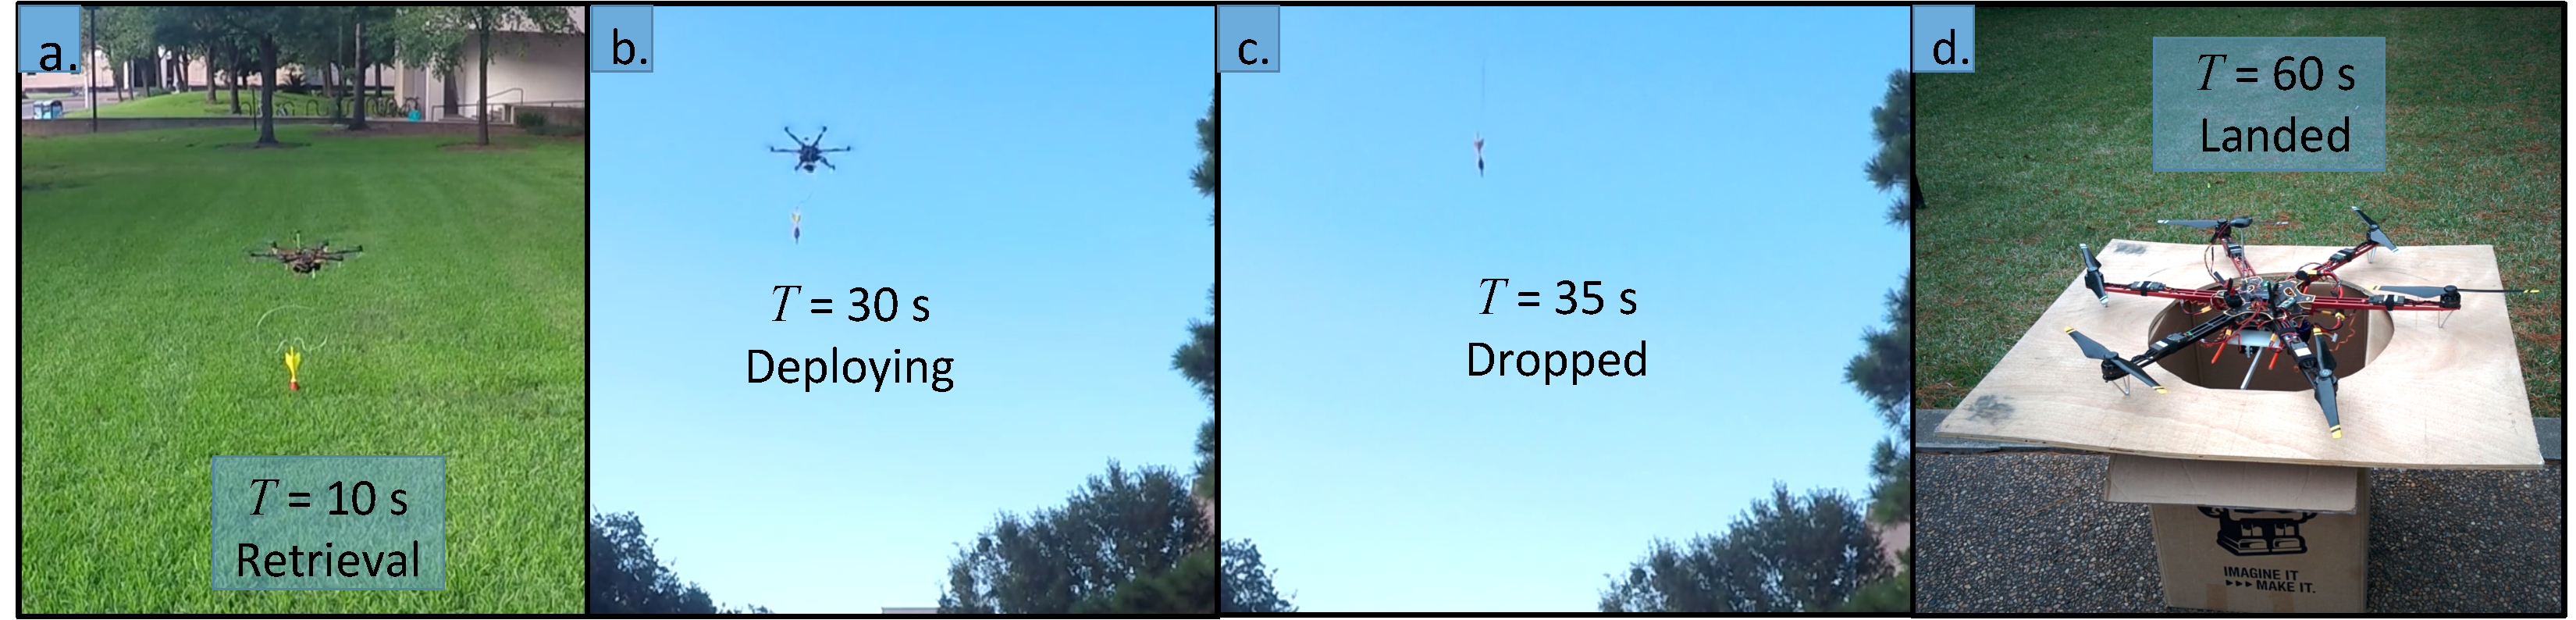
\includegraphics[width=\columnwidth]{SeismicDart_DR.pdf}}
 \caption{SmartDart retrieval and redeployment  See video  attachment. 
 \label{fig:SeismicDart_DR}}
\end{figure}
 